\section{Introduction}

% It shows very briefly how can we proceed to execute
%some basic things like the event generation, reconstruction and data
%analysis. For more details on how AliRoot works and how the experimental
%data can be analyzed, I strongly recommend to read the AliRoot primer~\cite{ALIROOT:doc}
%(the present document is not a substitute of the ``AliRoot primer''
%but an introduction for beginners), and also the AliEn pages~\cite{ALIEN:alien}
%or go directly to the code in~\cite{ALIROOT:svn}. 
%For detailed information on the EMCAL code you can go to the EMCAL offline pages (work in progress)~\cite{EMCAL:doc}.

%I will assume that you have already AliRoot and its environment properly
%installed in your machine, if not, look at \cite{ALIROOT:doc} or to the offline installation page \cite{ALIROOT:install}.
%If you type ``cd \$ALICE\_ROOT'', you will find all the AliRoot
%code. In the directories ``\$ALICE\_ROOT/macros'' and ``\$ALICE\_ROOT/EMCAL/macros'', you will find different examples of macros. All the EMCal
%code is in ``\$ALICE\_ROOT/EMCAL'', in case you want to study
%thoroughly how the simulation, reconstruction and analysis software
%code of the calorimeter work. 

%If we want to generate some data (realistic physics data or just single
%particle to study the performance of the ALICE detectors) or read
%real experimental data, and analyze it with AliRoot, we have to pass
%through three steps: \textbf{simulation}, \textbf{reconstruction}
%and \textbf{analysis}. This steps are explained in the next sections. 

This document is addressed to those who want to work with the EMCal data. It explains the different steps to have the data taken ready to be analyzed: geometrical description of the detector, how to get the calibration, how works the simulation and reconstruction of the data and how to access the analysis objects, ESDs and AODs.\\

For introduction on the detectors, the TDR's of the EMCal and DCal can be found in ~\cite{EMCalTDR,DCalTDR}.
For a fast introduction on the code and how it works you can have a look to the EMCal for beginners guide \cite{EMCAL:beginners}. Some other interesting references are the AliRoot primer~\cite{ALIROOT:doc}, the offline AliRoot page \cite{ALIROOT}, and the installation page from Dario Berzano \cite{ALIROOT:berzano}.\\

In general, a lot of information can be found in many twikis collected in the main EMCal twiki page that can be found here~\cite{EMCAL:MainTwiki} and also is interesting to point to the main EMCal offline twiki that can be found here~\cite{EMCAL:OffTwiki}.

\subsection{Mechanical description of the EMCAL}
(Federico Ronchetti)\\

The chosen technology is a layered Pb-scintillator sampling calorimeter with a longitudinal pitch of 1.44 mm Pb and 1.76 mm scintillator with longitudinal 
Wavelength Shifting Fiber (WLS) light collection, see the EMCal TDR~\cite{EMCalTDR}. The full detector spans $\eta$ = -0.7 to $\eta$= 0.7 with an azimuthal acceptance of $\Delta\phi~107^\circ$ 
and is segmented into 12,288 towers, each of which is approximately projective in $\eta$ and $\phi$ to the interaction vertex. 
The towers are grouped into super modules of two types: full size which span $\Delta\phi=20^\circ$ (24 ($\phi$) $\times$48 ($\eta$) towers) and 1/3 size which span $\Delta\phi$ = 6.67$^\circ$  (8 ($\phi$) $\times$48 ($\eta$) towers). 
There are 10 full size and 2, 1/3-size super modules in the full detector acceptance (Fig. \ref{fig:emcal-full}). \\

\begin{figure}[ht]
\begin{center}
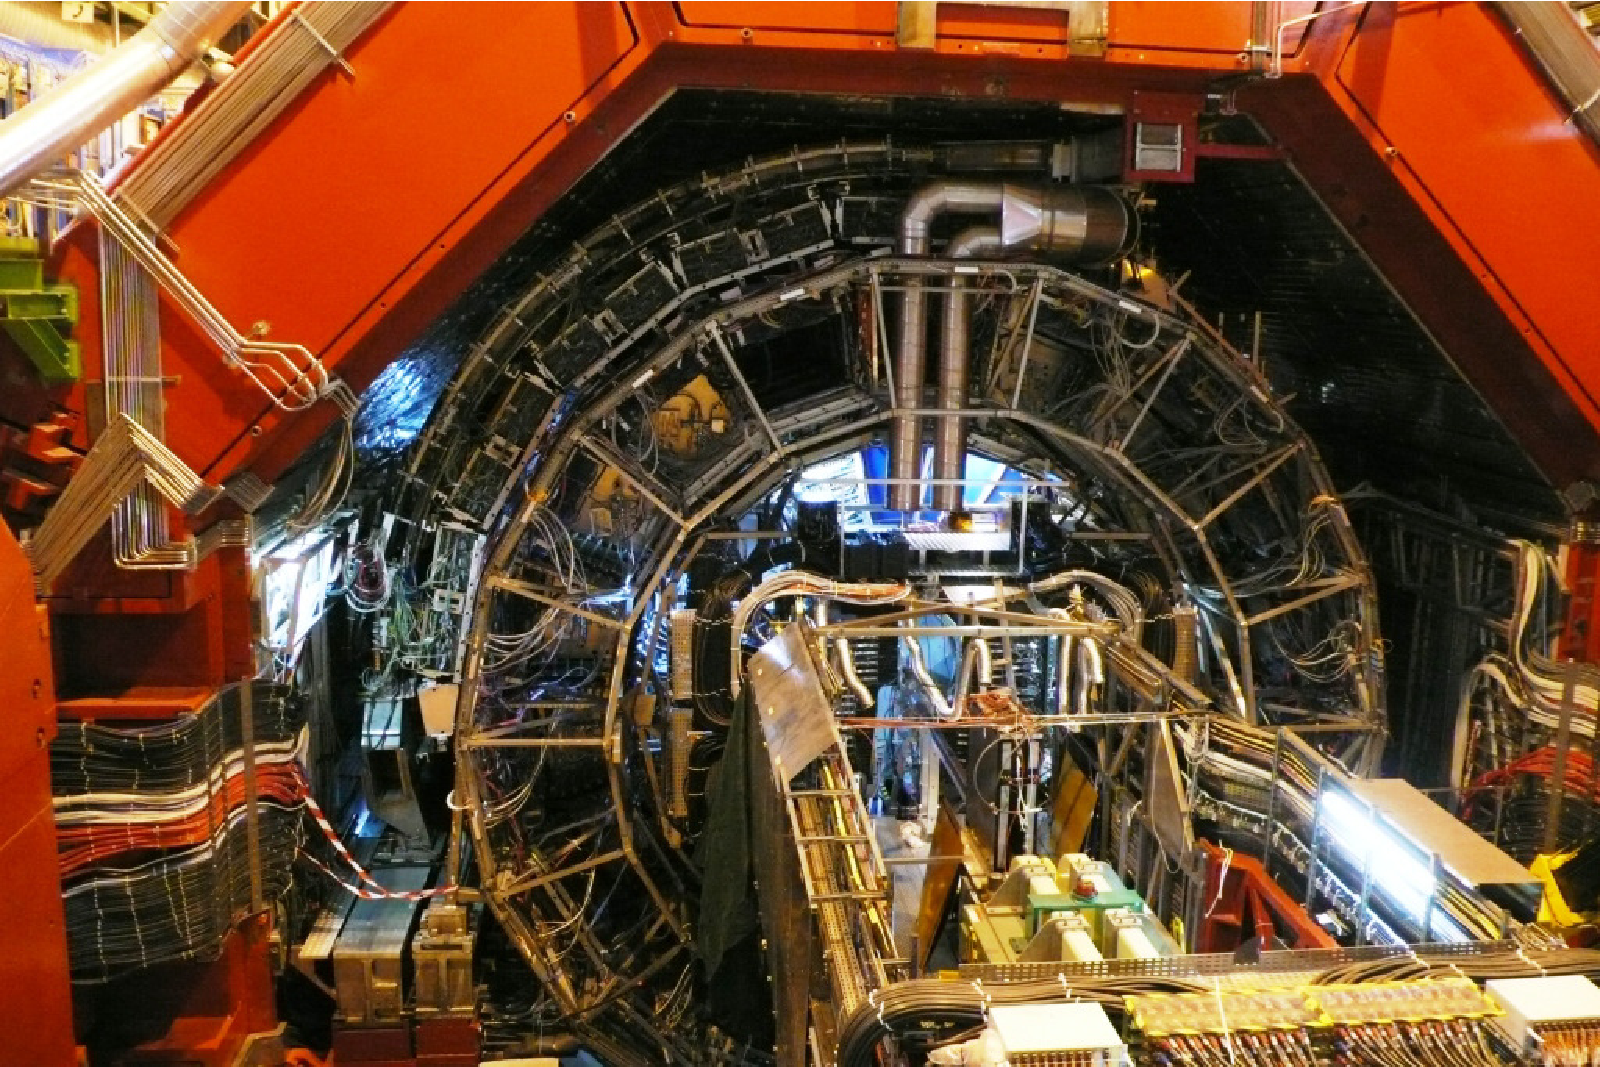
\includegraphics[width=1.0\textwidth]{figures/emcal-full.pdf}
\end{center}
\caption{\label{fig:emcal-full} Azimuthal view from the A-side (opposite to the di-muon arm) of the full EMCal as installed into the ALICE detector.
The two 1/3-size super-modules are visible at ~9 o'clock position.}
\end{figure}


In 2014, DCal extension was installed \cite{DCalTDR}, consisting of 6 super modules, with 2/3 the acceptance of an EMCal super-module (same acceptance in $\phi$ smaller in $\eta$ where 0.22$<|\eta|<$0.7,  24($\phi$)$\times$32 ($\eta$) towers) and 2 super-modules with 1/3 acceptance like for the EMCal. This extension covers 67 degrees in azimuth and same coverage in $\eta$ as the EMCal if one considers PHOS, although there is a gap of approx. 0.09 pseudo-rapidity units between PHOS and DCal super-modules, see Fig.~\ref{fig:dcal}. DCal is located opposite to EMCal, in azimuth, in the ALICE coordinate system EMCal is located at 80$<\phi <$187 degrees and DCal at 260$< \phi <$ 327 degrees. The total number of towers in DCal is 5,376.\\


\begin{figure}[ht]
\begin{center}
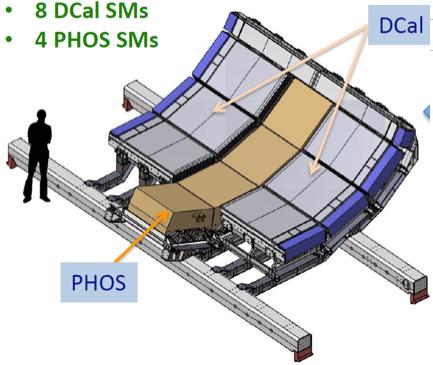
\includegraphics[width=0.5\textwidth]{figures/DCalPHOS.jpg}
\end{center}
\caption{\label{fig:dcal} Cartoon of the DCal+PHOS configuration in super-modules.}
\end{figure}


The super module is the basic structural units of the calorimeter. 
These are the units handled as the detector is moved below ground and rigged during installation. 
Fig.~\ref{fig:emc-sm} 
%shows a super module with its external mechanical structure stripped away to illustrate the stacking of modules within the super module. 
shows a full size super module with $12\times24$ modules configured as 24 strip modules of 12 modules each. DCal super modules contain $12\times16$ modules, 16 strip modules of 12 modules each.
The supporting mechanical structure of the super module hides the stacking into a nearly projective geometry which can be inferred by the different tilt
of the strip modules from lower $\eta$ to higher $\eta$. %going from the left to the right part of the picture. 
The electronics integration pathways are also visible. 
Each full size super module is assembled from $12 \times 24$ = 288 modules arranged in 24 strip modules of 12 modules each. 

\begin{figure}[ht]
\begin{center}
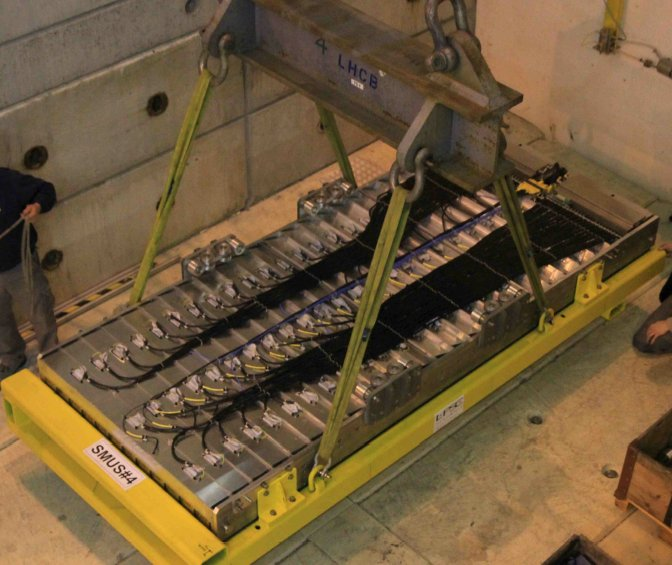
\includegraphics[width=1.0\textwidth]{figures/emc-sm.jpg}
\end{center}
\caption{\label{fig:emc-sm} View of one EMCal super-module during the installation into the ALICE detector. The cradle holds the 24 strip modules into a mechanically rigid unit.
Each strip module holds 12 unit modules. On the right side the two electronics crates are visible. }
\end{figure}

Each module has a rectangular cross section in the $\phi$ direction and a trapezoidal cross section in the $\eta$ direction with a full taper of 1.5$^\circ$. 
The resultant assembly of stacked strip modules is approximately projective with an average angle of incidence of less than 2$^\circ$ in $\eta$ and 
less than 5$^\circ$ in $\phi$. An assembled strip module is shown in Fig. \ref{fig:strip}.

\begin{figure}[ht]
\begin{center}
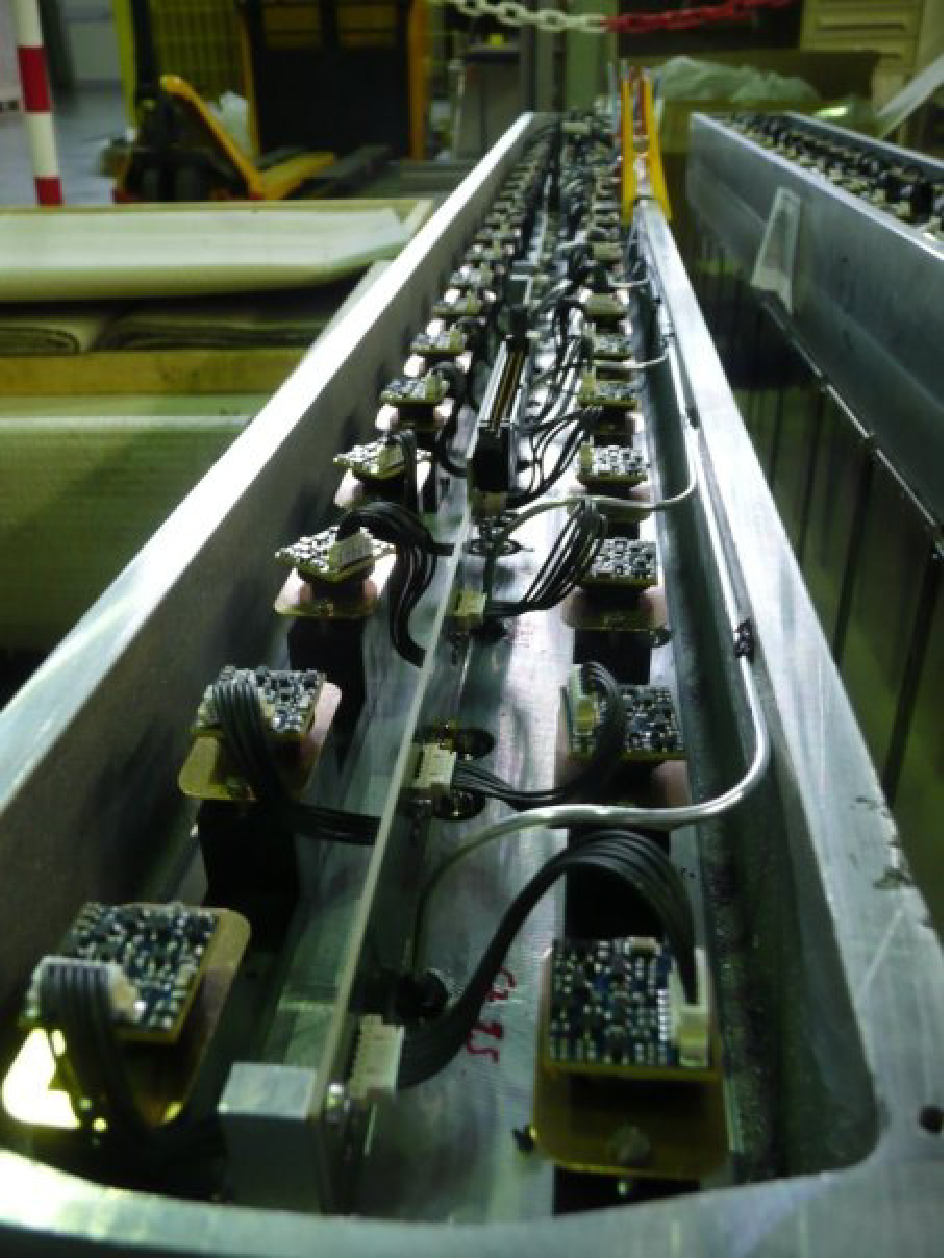
\includegraphics[width=0.5\textwidth]{figures/strip-module.pdf}
\end{center}
\caption{\label{fig:strip} View of a fully assembled strip module. The photo shows the APD+CSP package and copper shielding monunted light guide fixture. On the right part
of the photo the LED UV optical fiber distribution system is visible. Each strip module, is cabled via 3 T-Cards visible in the center of the assembly.}
\end{figure}

The smallest building block of the calorimeter is the individual module illustrated in Fig. \ref{fig:module}.
Each individual module contains $2\times 2$ = 4 towers built up from 77 alternating layers of 1.44 mm Pb and 1.76 mm polystyrene, 
injection molded scintillator. White, acid free, bond paper serves as a diffuse reflector on the scintillator 
surfaces while the scintillator edges are treated with TiO2 loaded reflector to provide tower to tower optical 
isolation and improve the transverse optical uniformity within a single tower. 
The Pb-scintillator stack in a module is secured in place by the static friction between individual 
layers under the overall  load of ~350 kg. The module is closed by a skin of 150 $\mu$m thick stainless 
steel screwed by flanges on all four transverse surfaces to corresponding front and rear aluminum  plates. 
This thin stainless skin is the only inert material between the active tower volumes. 
The internal pressure in the module is stabilized against thermal effects, 
mechanical relaxation and long term flow of the Pb and/or polystyrene by a customized 
array of 5 non-linear spring sets (Bellville washers) per module. 
In this way, each module is a self supporting unit with a stable mechanical lifetime of 
more than 20 years when held from its back surface in any orientation as when mounted in a strip module.

%\begin{figure}[ht]
%\begin{center}
%\end{center}
%\caption{\label{fig:module} 
%
%}
%\end{figure}


\begin{figure}[ht]
\begin{center}
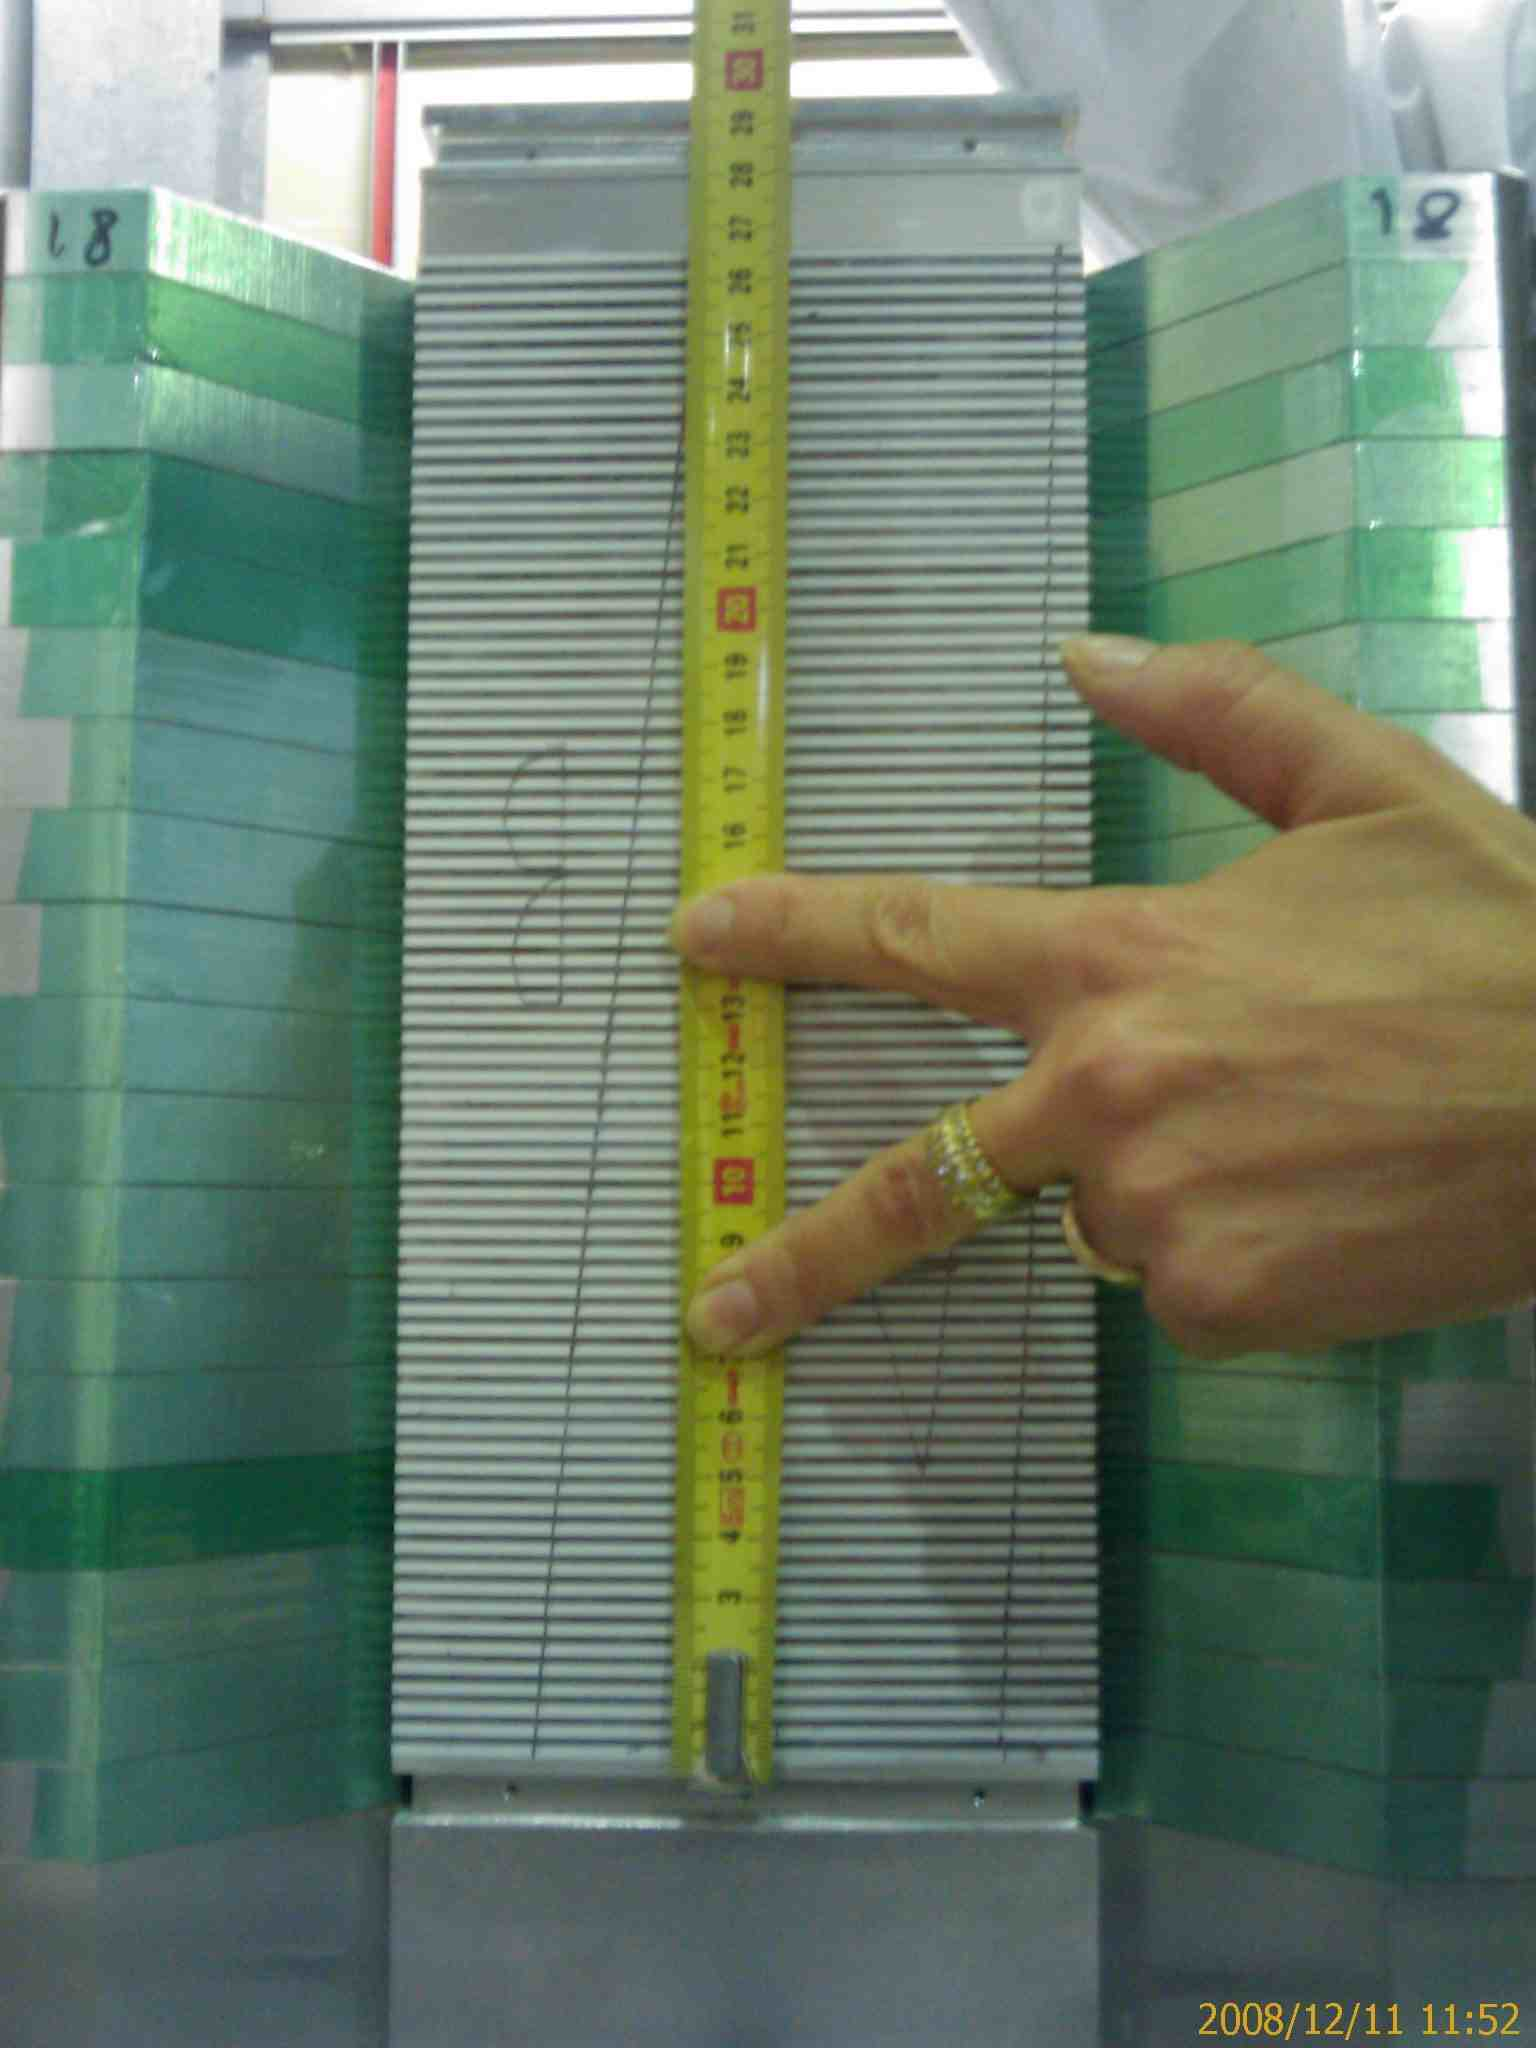
\includegraphics[width=0.45\textwidth]{figures/open-module.jpg}
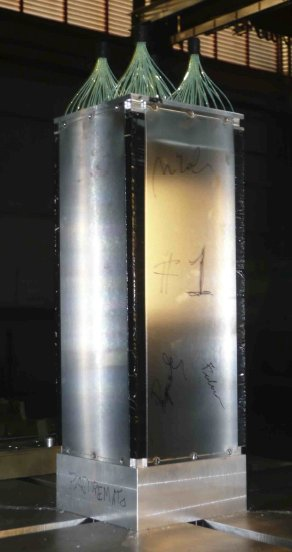
\includegraphics[width=0.32\textwidth]{figures/emc-module.jpg}
\end{center}
\caption{\label{fig:module} The first 1.5$^\circ$ tapered module of the EMCal generation II prototype produced in EU shown: Left: Internal Pb-scintillator sandwich of EMCal modules. Right: The module's internal compression is maintained by a set of 5 Bellville washers (non linear springs) acting between the top and bottom containment 
Al plates to prevent the delamination of the internal Pb-scintillator sandwich.
}
\end{figure}


All modules in the calorimeter are mechanically and dimensionally identical. The front face dimensions of the 
towers are $6\times6$ $cm^2$ resulting in individual tower acceptance of $\Delta\eta\times\Delta\phi=0.014\times0.014$ at $\eta$=0.
The EMCal design incorporates a moderate detector average active 
volume density of ~5.68 g/cm$^3$ which results from a 1:1.22 Pb to scintillator ratio by volume shown in Fig.~\ref{fig:module}. 
This results in a compact detector consistent with the EMCal integration volume at the chosen detector thickness of 20.1 radiation lengths. 
%Practical considerations, including the total assembly labor cost, 
%suggest reducing the total number of Pb/scintillator layers thus decreasing the sampling frequency. 

As described above, the super module is the basic building block of the calorimeter. 
Starting with 288 individual modules which are rather compact and heavy, the main engineering task is to create a super module structure which is rigid, 
with small deflections in any orientation yet does not require extensive, heavy external stiffening components that would reduce the volume available for the active detector. 
The solution adopted for the ALICE EMCal is to develop a super module crate which functions not as a box for the individual modules 
but rather an integrated structure in which the individual elements contribute to the overall stiffness. 
The super module crate is effectively a large I-beam in which the flanges are the long sides of the crate and the 24 rows of strip modules together. 
This configuration gives to the super module good stiffness for both the 9 o'clock and 10 o'clock locations. For the 12 o'clock location, 
the I-beam structure of the super module is augmented by a 1 mm thick stainless steel forward sheet (traction loaded), 
which controls the bending moment tending to open the crate main sides, and helps to limit deflection of strip modules. 
Ridges are provided on the interior surfaces of the crate to allow precision alignment of the strip modules at the correct angle. 
The stiffness given by this I-beam concept allows the use of non-magnetic light alloys for main parts of the super module crate. 
Parts of the super module crate will be made mainly from laminated 2024 aluminum alloy plates. 
The two main sides (flanges of the I-beam) of the crate will be assembled from 2 plates, 25 mm and 25 mm thick, 
bolted together and arranged so as to approximately follow the taper of the 20 degree sector boundary. Each of the 24 rows of a super module contain 12 modules as described above. 
Each of the modules is attached to a transverse beam by 3.4 mm diameter stainless steel screws. 
The 12 modules and the transverse beam form a strip module. The strip module is 1440 mm long, 120 mm wide, 410 mm thick. 
The total weight of the strip module is approximately 300 kg and like module, it is a self supporting unit. 
The transverse beam, which is the structural part of the strip module, is made from cast aluminum alloy 
with individual cavities along its length where the fibers emerging from towers are allowed to converge. 
The casting process is well suited to forming these cavities and the overall structure, saving considerable raw material and machining time. 

In addition to functioning as a convenient structural unit which offers no interference with the active volume of the detector 
and forming the web of the I-beam structure of the super module, the transverse beam of the strip module provides protection for the fibers, 
a structural mount for the light guide, APD and charge sensitive preamplifier and a light tight enclosure for these elements.


\subsection{Functional description of the EMCAL}

%**** need some additional info on PE APDs *********
%EMCAL basic units are cells/towers (Pb-scintillator sandwich of about 70 layers). We have 12 SuperModules (4 in 2010, 10 in 2011-2012) composed of 24 (phi direction) x 48 (eta direction) cells (except last 2 SuperModules made of 8 cells in phi direction). 

Particles traversing the calorimeter, in particular photons and electrons, will deposit energy in different towers. 
The EMCAL reconstruction measures such energy per tower, forms clusters of cells produced by a given particle, 
and if possible matches them with particles detected by the tracking detectors in front of EMCAL (charged particles).

Scintillation photons produced in each tower are captured by an array of 36 Kuraray, 
Y-11, double clad, WLS fibers that run longitudinally through the Pb/scintillator stack.
Each fiber terminates in an aluminized mirror at the front face end of the module and is integrated into a polished, 
circular group of 36 at the photo sensor end at the back of the module. 
The fiber bundles are pre-fabricated and inserted into the towers after the module mechanical assembly is completed. 
The 36 individual fibers are packed into a circular array 6.8 mm in diameter and held in place inside a custom injection 
molded grommet by Bicron BC-600 optical cement. An optical quality finish is applied to the assembled bundle using a diamond polishing machine. 
At the other end of the bundle, individual fibers are similarly polished and mirrored with a sputtered coat 
of aluminum thick enough to ensure the protection of the inner mirror. 
The response of the Al-coated fiber is considerably flatter with an overall increase in efficiency in the range of about 25\% in the vicinity of shower maximum 
(i.e. the location of the highest energy deposition for an electromagnetic shower).  
This number accounts for material immediately in front of the detector; which ranges between 0.4 and 0.8 radiation lengths, 
and assumes 5.5 - 6.0 radiation lengths for shower maximum for 10 GeV photons. 
At this depth in the detector, the mirrored fiber response is very uniform does not contribute to the non-linearity of the detector as a whole. 

Other factors which can significantly impact the electromagnetic performance of the calorimeter, 
include scintillator edge treatment and the density of the wavelength shifting fiber readout pattern and the material 
chosen for the interlayer diffuse reflector. For scintillator edge treatment and fiber density, advantage was taken from the 
extensive studies made by the LHCb collaboration for their ECAL. In particular, a diffuse reflector edge treatment was adopted, 
such as that obtained with Bicron Titanium Dioxide loaded white paint (BC622A) with a total fiber density of about one fiber per $cm^2$. 
In the case of the interlayer diffuse reflector, a white, acid free, bond paper was used in place of the Teflon based commercial TYVEK. 
While TYVEK produces slightly better surface reflectivity, its coefficient of friction is too low to permit its use in this 
design where the module's mechanical stability depends somewhat on the interlayer friction.
 
The 6.8 mm diameter fiber bundle from a given tower connects to the APD through a short light guide/diffuser 
with a square cross section of 7 mm $\times$ 7 mm that tapers slowly down to 4.5 mm $\times$ 4.5 mm as it mates (glued) 
to the 5 mm $\times$ 5 mm active area of the photo sensor. 
The 4 pre-fabricated fiber bundles are inserted into the 
towers of a single module. 

The selected photo sensor is the Hamamatsu S8664-55 Avalanche Photo Diode.
% ************
This photodiode has a peak spectral response at a wavelength of 585 nm compared to an emission peak of 476 nm for the Y-11 fibers. 
However, both the spectral response and the quantum efficiency of the APD are quite broad with the latter dropping from the maximum by only ~5\% at the WLS fiber emission peak. 
At this wavelength, the manufacturer's specification gives a quantum efficiency of 80\%. 
